\documentclass[a4paper,12pt,twoside]{report}
\usepackage[left=2cm,right=2cm,top=2cm,bottom=3cm]{geometry}

\usepackage[utf8]{inputenc}
\usepackage{amsmath}
\usepackage[spanish, es-tabla]{babel}
\usepackage{amsfonts}
\usepackage{amssymb}
\usepackage{multirow, array} 
\usepackage{chngcntr}
\usepackage{graphicx}
\usepackage{subfig}
\usepackage{cite}
\usepackage{adjustbox}
\usepackage[table]{xcolor}
\usepackage{braket}
\usepackage{lipsum}

\usepackage{color}   %May be necessary if you want to color links
\usepackage{hyperref}
\hypersetup{
    colorlinks=true,
    linkcolor=black,
    urlcolor=magenta,
    citecolor=blue
}

\title{}
\begin{document}
\begin{center}
\thispagestyle{empty}
\fontsize{12pt}{12pt}\selectfont 

%%%%%%%%%%%%%%%%%%% PORTADA %%%%%%%%%%%%%%%%%%%%%%%%


\textbf {\huge Calibración del espectrografo EShel- II PF0011}
%\huge

\vspace{3cm}


{\large \textbf{Autor:}}

\vspace{0.5cm}

\large Jesús Alberto Sánchez Villafrades$^{1,2}$

\vspace{3cm}

{\large \textbf{Director}}\\

\vspace{0.5cm}

{\large Director: Luis Alberto Núñez$^{1,2}$}\\

\vspace{0.5cm}

{\large \textbf{Codirector}}\\

\vspace{0.5cm}

{\large Juan Pablo Uchima Tamayo $^{3}$}

\vspace{3cm}

\normalsize

\large Propuesta de trabajo de grado para optar al t\'itulo de F\'isico


\vspace{4cm}



\large $^1$Grupo de Investigaci\'on en Relatividad y Gravitaci\'on GIRG \\
\large  $^2$Grupo Halley de Astronom\'ia y Ciencias Aeroespaciales \\
\large  $^3$Universidad de la Serena \\
\large  Escuela de Física - 2020
  \end{center}
  
\newpage
%%%%%%%%%%%%%%%%%%%%%%FIN  DE LA PORTADA    %%%
%\leavevmode\thispagestyle{empty}\newpage

\newpage

%------------- Documento --------------
%%%%%%%%%%% PARA LA TESIS FINAL
\pagenumbering{roman}
\setcounter{page}{2}
%\input{Nota.tex}
%\input{Autorización}
%\addcontentsline{toc}{chapter}{Dedicatoria}
%\input{Dedicatoria.tex}
%\addcontentsline{toc}{chapter}{Agradecimientos}
%\input{Agradecimientos.tex}

%%%%%%%%%%%%%%%%%%%%%%%%%%%%%%%%%%%%%%%%%%%%%%%%%%%%%
\tableofcontents % indice de contenidos
\cleardoublepage
%\addcontentsline{toc}{chapter}{Lista de figuras}
\listoffigures % indice de figuras
%\addcontentsline{toc}{chapter}{Lista de tablas}
\listoftables % indice de tablas
%\addcontentsline{toc}{chapter}{Lista de símbolos}
%\input{Symbols/Symbols}
%\addcontentsline{toc}{chapter}{Resumen}
%\addcontentsline{toc}{chapter}{RESUMEN}
\newpage
\chapter*{RESUMEN}
\label{sec:resum}

\textbf{TÍTULO:}Calibración\\

\textbf{AUTORA:} Jesús Alberto Sánchez Villafrades\\

\textbf{PALABRAS CLAVES: } jjjjjjjjjjjjjjj\\


%\addcontentsline{toc}{chapter}{Abstract}
%\addcontentsline{toc}{chapter}{Abstract}
\newpage
\chapter*{ABSCTRACT}
\label{sec:abst}

\textbf{TITLE:} .........\\

\textbf{AUTHOR:} .....................\\

\textbf{KEYWORDS: } ................\\


%en el proceso de formación de cascadas aéreas extensas (EAS), más específicamente,

%%%%%%%%%%%%%%%%%%%%%%%%%%%%%%%%%%%%%%%%%%%%%%%%%%%%%Cambio de Numeración
\newpage
\pagenumbering{arabic}
\setcounter{page}{1}

\addcontentsline{toc}{chapter}{INTRODUCCIÓN}
\newpage
\chapter*{INTRODUCCIÓN}
\label{sec:intro}

\lipsum{1-3}


\newpage
\chapter{Objetivos}

%%%%%%%%%%%%%%%%%%%%%%%%%%%%%%%%%%%%%%%%%%%%%%%%%%%%%%%%%%%%%%%%%%%%%%%%%%%%%%%%%%%%%%%%%%%%%

\begin{itemize}
\item \textbf{Objetivo General}

Realizar el montaje, calibración y puesta en funcionamiento de ESPECTRÓGRAFO eShel II con el que cuenta el Grupo Halley de Astronomía y Ciencias Aeroespaciales de la Universidad Industrial de Santander.\\

\item \textbf{Objetivos Específicos}
\end{itemize}

\begin{itemize}


\item Verificar el enfoque del lente colimador del espectrógrafo eShel II verificándolos con lineas de lamparas de emisión.

%Diseño y realización del montaje cámara SBIG 6303E y el espectrógrafo eShel II para verificar las lámparas de calibración Led, Tungsteno y Torio-Argón 
%Pedirle a Pisco los diseños.

\item Realizar la calibración pixel-Longitud de onda mediante el software IRAF, usando lamparas de calibración con espectros conocidos.

\item Realizar el análisis de el espectro dos estrellas de la bóveda celeste como forma de validación de la metodología.

 \item Realizar los cálculos teórico y experimentales de la masa de aire para la ciudad de Bucaramanga a partir de toma de datos con una estrella, para el análisis de la función de dispersión de punto.
%función de dispersión de punto

\end{itemize}
\newpage

\newpage
\chapter{Marco teórico}

La espectroscopia estudia la interacción entre la radiación electromagnética y la materia,en astronomía esta radiación es emitida por estrellas y otros objetos celestes y al ser dispersada brinda mucha información de la fuente que la genero.\\
Para el caso del espectro visible esta Luz puede ser dispersada usando un prisma mediante el fenómeno de refracción o usando una rejilla de difracción, estos espectros dan información importante de las características físicas del objeto que las emite,están directamente relacionadas con la temperatura superficial del objeto así como con su composición química. Usando Efecto Doppler se puede tener información de la velocidad de rotación y traslación además de densidad y presión. \cite{utilidad}\\



\section {Principios de la espectroscopia.}
Todo elemento que  irradie luz presenta en esta luz información detallada de las propiedades constituyentes de dicho elemento así como su temperatura, esta luz esta compuesta de múltiples longitudes de onda que son separadas y se pueden observar en un sensor ccd en forma de linea espectral, que es la distribución de  la intensidad en función de la longitud de onda o la frecuencia  de luz dispersada.

\subsection {Espectros y lineas espectrales.}

Históricamente las lineas espectrales fueron llamadas así ya que se  presenta como lineas de obscuridad o luminosidad en la salida de un espectroscopio luego de la dispersión, por esto la forma de las lineas dependen del instrumento que se este utilizando.\\
Estas lineas son de origen cuántico y se generan por la transición de 2 niveles de energía, estos puede dividirse en 3 tipos,las lineas espectrales continuas ,de emisión y las de absorción.\cite{troccoli}


\textbf{Espectro Continuo:}
Se define un espectro continuo cuando la franja de colores  pasa de un color a otro sin ninguna interrupción de franjas negras entra color y color como se presente en la figura 1, se puede observar esto con la luz blanca y en general cualquier solido o gas sometido a altas presiones o temperaturas presente un espectro continuo.


\begin{figure}[htb!]
\centering

\includegraphics[width=0.7\textwidth]{images/1.png}
\caption[Espectro continuo.]{Espectro continuo.\cite{libro}}
 \label{fig2}
\end{figure}

\textbf{Espectro de emisión :} Un gas a baja presión y excitado a altas temperaturas produce un espectro de emisión,estos espectros constan de rayas de diversos colores separadas por amplias zonas  negras en las que no se observa luz ver figura 2. Este tipo de espectro se da cuando los electrones en los átomos de estos gases excitados absorben energía de la fuente que los esta excitando  y saltan a orbitas superiores , la emisión tiene lugar cuando los electrones caen a niveles mas bajos emitiendo este exceso de energía en forma de fotones con una frecuencia característica propia de cada elemento.


 \begin{figure}[htb!]
\centering
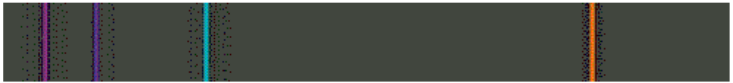
\includegraphics[width=0.7\textwidth]{images/2.png}
\caption[Descripción versión comprimida]{El espectro de emisión del hidrógeno \cite{articulo1}}
 \label{fig3}
\end{figure}


\textbf{Espectro de absorción :} Este tipo de espectro se da cuando se hace pasar luz blanca a través de un gas frío a baja presión, el espectro que se observa presenta un fondo de color con franjas negras, con la característica principal de que las lineas de absorción aparecen en el mismo lugar que las lineas de emisión.\\
En astronomía las fuente luminosa generalmente es una estrella, la luz proveniente de la estrella atraviesa capas de gas propia de la atmósfera, las lineas de absorción dependerán estrictamente de la composición química del gas, esta absolverá fotones de una u otra longitud de onda dejando las franjas obscuras características de espectro de absorción.


\begin{figure}[htb!]
\centering
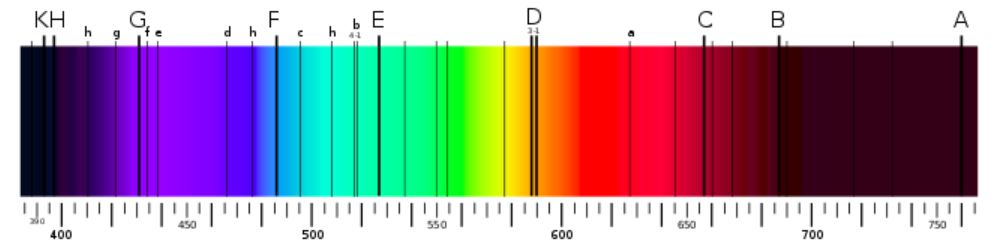
\includegraphics[width=0.7\textwidth]{images/3.png}
\caption[Descripción versión comprimida]{Espectro solar en el que se aprecian las líneas principales de von Fraunhofer. \cite{articulo1}}
 \label{fig4}
\end{figure}

%falta citar de https://culturacientifica.com/2019/08/13/los-espectros-de-absorcion-de-los-gases/

Los anteriores espectros tienen su explicación en las leyes de kirchof  que se presentan a continuación.

-Un espectro continuo se produce por un un solido incandescente o un gas a alta presión.

-Un espectro de emisión se produce por un gas incandescente a baja presión.

- Cuando se hace pasar luz blanca a través de un gas a baja presión y baja temperatura se produce un espectro de emisión.

\subsection {Radiación de cuerpo negro}
Es bien conocido el fenómeno por el cual todos los cuerpos que se encuentran por encima del cero absoluto presentan radiación electromagnética, a altas temperaturas se habla de incandescencia pues las longitudes de onda de emisión se encuentran en el espectro visible (entre 400 y 700 nm) aun a bajas temperaturas  el objeto seguirá irradiando pero ahora en el infrarroja (longitudes de onda superiores a 700 nm).\cite{libro2} \\
Kirchoff propuso en 1860   una hipótesis  de radiación para los cuerpo en equilibrio , la denomino radiación de cuerpo negro, esta muestra como la radiación tiene un patrón regular que depende de la temperatura.Mas tarde  Wein y Plank  hicieron el desarrollo matemático e este fenómeno, que se puede modelar como:


\begin{equation}
    \lambda_{max}=\frac{0.002898}{T}
\end{equation}


Donde $ \lambda$ es la longitud de onda máxima emitida por el cuerpo y T es la temperatura en grados Kelvin.\\

\noindent \textbf{Ley de desplazamiento de Wien:}Durante el año 1893 Wien basándose en argumentos estadístico dedujo que la distribución normal de radiación, como era conocida hasta la fecha se modelaba  con la expresión:  


\begin{equation}
    I(\nu,T)=\nu^3 f \left(\frac{\nu}{T}\right)
\end{equation}


\noindent Donde $f\left(\frac{\nu}{T}\right)$ es desconocida pero solo puede depender de $\nu$ y de T.\\
Sin embargo Wien usando los datos de los experimentos realizados en la época pudo llegar a una expresión mas detallada para la ecuación  (2).  


\begin{equation}
    I(\nu,T)= a \nu^{3} e^{-b(\frac{\nu}{T})}
\end{equation}{}


\noindent Donde a y b son constantes que se determinan durante el experimento.\\
Esta expresión modelaba muy bien los experimentos  reproducidos en la época y daba una explicación satisfactoria a los resultados empíricos que demostraban que la frecuencia de radiación mas intensa emitida por un cuerpo negro $\nu_{max}$ aumenta linealmente con la temperatura.

\begin{figure}[htb!]
\centering
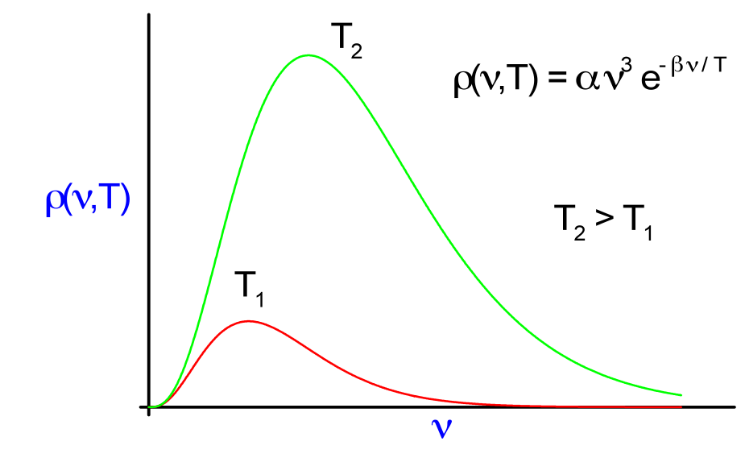
\includegraphics[width=0.6\textwidth]{images/5.png}
\caption[Descripción versión comprimida]{Wien propuso la expresión para la distribución normal de radiación que predice el pico de la distribución de corriente lineal con la la temperatura T.\cite{plank}}
 \label{fig1}
\end{figure}

\noindent \textbf{La deducción de Planck:}Para el año 1900 Otto Lummer y Ernst Pringsheim junto con otros 2 investigadores Heinrich Rubens y Ferdinand Kurlbarm realizaron múltiples experimentos y notaron que la ecuación de Wien (1.3) no concordaba con los experimentos a frecuencias bajas, a estas frecuencias la distribución normal de radiación notaron que eran directamente proporcional al cuadrado de la frecuencia por la temperatura.

\begin{equation}
    I(\nu,T) \sim \nu^{2} T
\end{equation}{}

\noindent Plank notando que la ley de Wien no era valida a frecuencias bajas e interpolando las ecuaciones (1.3) y (1.4) Plank propuso una expresión valida para frecuencias frecuencias altas y bajas.

\begin{equation}
    I(\nu,T)= \frac{2 h \nu^3}{c^3}\frac{1}{e^\frac{h\nu}{KT}-1}  
\end{equation}{}


\begin{figure}[htb!]
\centering
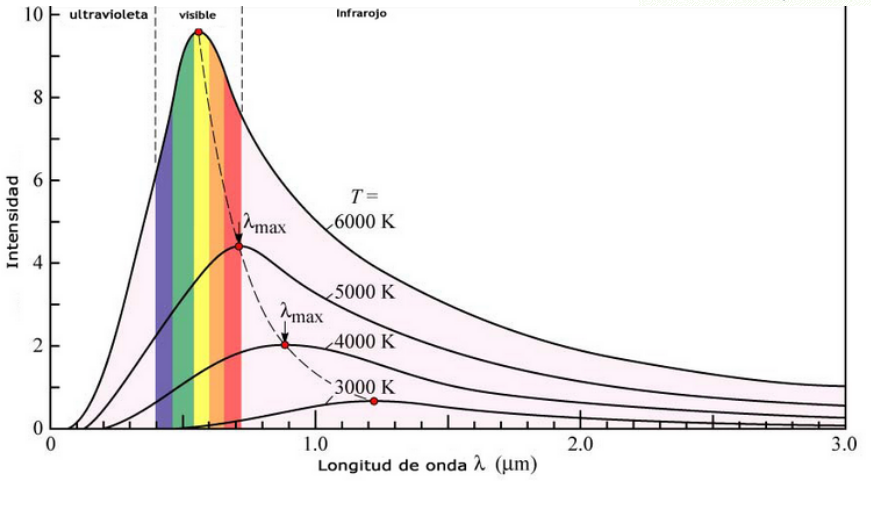
\includegraphics[width=0.8\textwidth]{images/6.png}
\caption[Descripción versión comprimida]{Función de radiación de Planck\cite{gra6}}
 \label{fig2}
\end{figure}




\noindent Esta deducción teórica en la gráfica \ref{fig2} explica la intensidad de radiación en función de la longitud de onda y la temperatura.Para proponer este resultado Planck se alejo de las teorias clasicas y propuso una teoria revolucionaria, Planck supuso osciladores con una frecuancia natural $\nu$ que solo podian obsorven o emitir energia de forma discreta en paquetes a los que llamo cuantos.
\begin{equation}
    E= nh\nu , n=1,2,3,4...
\end{equation}{}

\noindent Donde $h$ se conoce como la constante de Planck, esta constante puede ser hallada mediante la función experimental y el valor aceptado actualmente es $h=6.62607x10^{-34} Js$.



\subsection {Información contenida en las lineas espectrales}
\newline
\noindent \textbf{El Continuo}\\

\noindent El nivel de continuidad $I_c$ o "Continuo" corresponde al curso de la intensidad de la radiación sobre la longitud de onda (siempre aumentando de izquierda a derecha), que es limpiada o suavizada por la existencia de lineas de absorción o emisión (curva azul). Siendo así podemos definir el continuo como toda el área entre el eje de la longitud de onda y el nivel de continuidad.  

\noindent Físicamente el continuo se ve representado con el modelo teórico de cuerpo negro que a su vez es un modelo  ideal no existente en la naturaleza.\\

\begin{figure}[htb!]
\centering
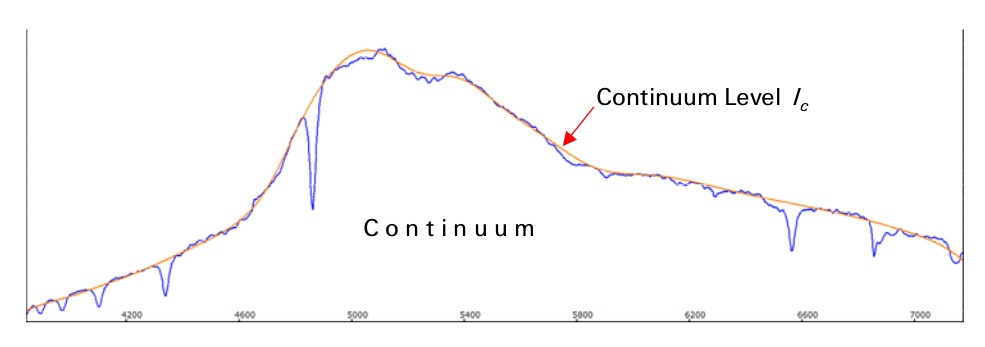
\includegraphics[width=0.9\textwidth]{images/8.jpeg}
\caption[Descripción versión comprimida]{nivel de continuidad $I_c$\cite{libro}}
 \label{fig2}
\end{figure}

\newpage


\noindent \textbf{Forma y características de las lineas espectrales.}\\\\

\noindent Las lineas de absorción o emisión se representan como como distribuciones de tipo Gausiano con un ancho definido y un grado de saturación que depende de que tanto atraviese o atraviese el continuo.
Las lineas espectrales de emisión se identifican como elevaciones desde el nivel de continuidad y las lineas de absorción en sentido opuesto desde la linea de continuidad.

\begin{figure}[htb!]
\centering
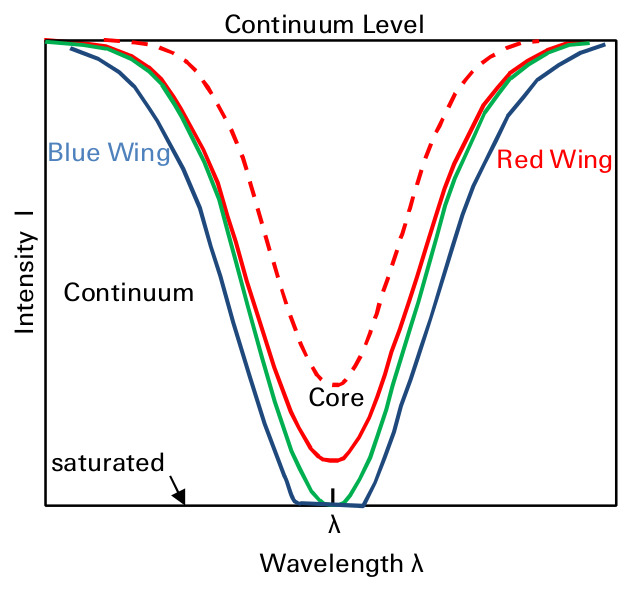
\includegraphics[width=0.48\textwidth]{images/9.jpeg}
\caption[Descripción versión comprimida]{Lineas de absorción con diferentes anchuras he intensidades penetrando la linea del continuo.\cite{libro}}
 \label{fig2}
\end{figure}

\noindent Se puede notar que los perfiles rojos son ambos insaturados, el verde solo toca un punto del eje de la longitud de onda esta saturado y el azul sobresaturado. A la base de la linea espectral se le conoce como núcleo de la linea y a sus extremos las alas, el ala de longitud de onda corta se llama ala azul y el longitud de onda larga ala roja.
\newpage




\noindent \textbf{Información contenida en las lineas espectrales}\\

\noindent  Existen pocos objetos en el cielo que presentan un espectro aproximadamente continuo, generalmente se observan lineas de emisión o absorción en el continuo de los espectros analizados y es precisamente en estas discontinuidades las que esconden información característica del objeto que esta emitiendo la luz dispersada.A continuación presentamos algunos procesos físicos que influencian en la formación de la linea espectral y por tal motivo son medibles analizando la deformación.

\begin{itemize}
    \item \textbf{Velocidad de rotación:} Las estrellas al igual que los planetas presentas rotación,esta velocidad de rotación de las estrellas ensancha y aplana su espectro pudiéndose medir esta velocidad analizando  estos ensanchamientos.
    \item \textbf{Temperatura y densidad de la atmósfera:}Las transiciones atómicas que producen las lineas espectrales se dan a temperaturas características propias de los elementos en los que se esta dando la transición, las lineas espectrales amplían la lineas haciendo posible la medición física de la temperatura superficial del objeto fuente.
    \item \textbf{Campos magnéticos fuertes:}Los campos magnéticos fuertes como las manchas solares producen una división y un desplazamiento en las lineas espectrales.
    \item \textbf{Velocidad de radial:}Las estrellas como los planetas presentan un movimiento 
    
    
    
    
    
    
    
    
\end{itemize}{}





\subsection {Clasificación espectral}



%http://www.quimicafisica.com/radiacion-cuerpo-negro-hipotesis-planck.html







\subsection {Diagramas de Hertzsprung-Russell}


\noindent La espectroscopia permitió la construcción del diagrama Hertzsprung-Russell, el cual se desarrollo inicialmente en la Universidad de Harvard.
Este diagrama muestra la etapa de evolución de las estrellas con las líneas espectrales que señala el estado de los elementos químicos presentes en ellas. La figura 2.3 muestra como se relacionan las estrellas en tamaño, color, luminosidad, clase espectral y la magnitud absoluta. Cada punto en este diagrama representa una estrella en el firmamento, cuya magnitud y clase espectral absoluta han sido determinadas. Los datos se agrupan en: estrellas de secuencia principal, supergigantes, gigantes y enanas
blancas.


%\subsection {Lineas de franhofer}


\subsection{Instrumentación}

 \noindent Para cumplir con los objetivos propuestos de tendrán que tomar espectros ya sea de lamparas de laboratorio con espectros conocidos o de estrellas, para esto se tendrá que usar y conocer las características de los instrumentos a utilizar, estos instrumentos hacen parte del complejo astronómico de grupo Halley de l universidad Industrial de Santander.\\

\noindent \textbf{ Telescopio CDK 17 (corrected Dall-kirkham)}\\

\noindent El telescopio CDK 17 (corrected Dall-kirkham) es un telescopio de tubo ópticoo de diseño abierto, hecho en fibra de carbono con un paso de 43 kg, cuenta con 2 lentes de 90 mm (aplanadores de campo) y 2 espejos. 
Un espejo primario elipsoidal con una apertura de 432 mm y una relación focal de f/2,6 y un espejo secundario con una apertura de 159 mm con forma esférica.\\
Posee un enfocador Hedrik 3.5 y tres ventiladores en la parte inferior y 4 en las laterales del tubo óptico, todo esto acoplado a una montura ecuatorial Paramount ME II.\\
La montura Paramout ME II tiene un eje de contrapeso DEC 47 CM  de largo y 48 mm de diametro, 2 contrapesos de 14 Kg, un rodamiento de declinacion de 48 puntos de contacto, con una capacidad de carga de 140 Kg.\\


\noindent \textbf{Espectrógrafo  eShell II }\\

\noindent El espectrógrafo eShell de la compañía Francesa Shelyak es un espectrógrafo de dispersión cruzada, eso quiere decir que la primera dispersión se realiza mediante un rejilla tipo echell  o "escalera" que típicamente utiliza ordenes altos entre el orden 32-52, 21 ordenes en total y posee un prisma como segundo dispersor que se encarga de separar los diferentes ordenes, esto permite combinar un alta resolución y una gran cobertura del dominio espectral.
El dispersor cruzado posee un foco de $f=125 mn$ un colimador de $\frac{f}{5}$ y un rango de operacion entre 450 y 700 nm.\\
La luz de los objetos de interés es enfocada por el telescopio y dirigida a una fibra óptica de $50\mu$, este fibra dirige la luz al espectrógrafo quien la dispersa y luego de esto esta luz dispersada es capturada por la cámara de guía que para nuestro caso es la cámara SBIG.\cite{echell}\\

\noindent El Instrumento completo incluye:

\begin{itemize}
    \item Espectrógrafo tipo Echell.
    \item Unidad de calibración con una lampara LED, una lampara de  Tungsteno y lampara de Torio-Argón.
    \item Una fibra óptica de guía de $50 \mu m$ conectada del acople del telescopio al espectrógrafo.
    \item Una fibra óptica de calibración de $200 \mu m$ conectada de la unidad de calibración al acople del telescopio.
    \item Una unidad de acople al telescopio donde se conecta la cámara guía.
\end{itemize}{}



\noindent \textbf{Cámara STXL-6303E }\\

\noindent Esta cámara cuenta con un sensor CCD de 16 Mega píxeles con adaptador de rueda de filtros micrométrica y autoguiado incorporado, para la disminución de ruido en las imágenes la cámara posee un enfriamiento mediante celdas Peltier de -60 grados Celcius, también posee un acople para óptica adaptativa así como un obturador de iluminación uniforme.A continuación se presenta información técnica detallada del censor y la cámara.

\begin{figure}[htb!]
\centering
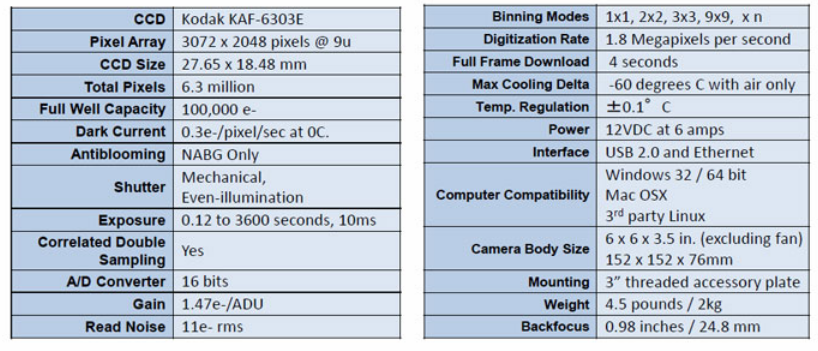
\includegraphics[width=0.8\textwidth]{images/7.png}
\caption[Espectro continuo.]{Ficha tecnica Camara SBIG STXL-6303E\cite{gra7}}
 \label{fig2}
\end{figure}




\newpage
\chapter{Metodología}


\subsection{Fase de lectura}
Para la realización de la calibración del espectrógrafo eShel II se 

\subsection{Montaje experimental  Espectrógrafo-Cámara-Telescopio.}

\subsection{Adquisición de datos}

\subsection{Procesamiento de datos}

\subsection{Evaluación de los resultados y validación de la metodología}

\begin{itemize}

\item[1] Montaje del espectrógrafo con sus respectivo modulo de calibración y acople al telescopio.

\item[2] hacer el calculo de forma experimental de la rendija del espejo que permite el paso de luz al espectrógrafo.

\item[3] Realizar la captura de imágenes limpias de diferentes lamparas de emisión de laboratorio con el fin de garantizar que los elementos dispersores del espectrógrafo estén alineados con la cámara y se puedan reproducir espectros conocidos.

\item[3] Se calibrara la Montura robotizada PARAMOUNT  usando el software T-Point para garantizar un correcto apunte del telescopio al objeto de interés.



 
\end{itemize}

%%%%%%%%%%%%%%%%%%%%%%%%%%%%%%%%%%%%%%%%%%%%%%%%%%%%%%%%%%%%%%%%%%%%%%%%%%%%%%%%%%%%%%%%%%%%%%


%%%%%%%%%%%%%%%%%%%%%%%%%%%%%%%%%%%%%%%%%%%%%%%%%%%%%%%%%%%%%%%%%%%%%%%%%%%%%%%%%%%%%%%%%%%%%%
\section{Cronograma de Actividades}	
%%%%%%%%%%%%%%%%%%%%%%%%%%%%%%%%%%%%%%%%%%%%%%%%%%%%%%%%%%%%%%%%%%%%%%%%%%%%%%%%%%%%%%%%%%%%%%


\begin{center}
{\small
\begin{tabular}{|c|c|c|c|c|c|c|c|}
\hline

\textbf{Mes}/\textbf{Actividad}&\textbf{Act 1.1}&\textbf{Act 1.2}
&\textbf{Act 1.3}&\textbf{Act 2}&\textbf{Act 3}&\textbf{Act 4}&\textbf{Act 5}\\

\hline

Enero&$\bigotimes$&&&&&&\\

\hline

Febrero&$\bigotimes$&$\bigotimes$&&&&&\\

\hline

Marzo&&$\bigotimes$&$\bigotimes$&&&&\\

\hline

Abril&&&$\bigotimes$&&&&\\

\hline

Mayo&&&$\bigotimes$&$\bigotimes$&&&\\

\hline

Junio&&&$\bigotimes$&$\bigotimes$&&&\\

\hline
Julio&&&$\bigotimes$&$\bigotimes$&$\bigotimes$&&$\bigotimes$\\

\hline

Agosto&&&&&$\bigotimes$&$\bigotimes$&\\

\hline 

Septiembre&&&&&&&$\bigotimes$\\

\hline
Octubre&&&&&&&$\bigotimes$\\
\hline

\end{tabular}
}
\end{center}
\newpage
\chapter{CONCLUSIONES}

\lipsum{1-2}
%\input{chapters/APENDICE_A.tex}
%\input{chapters/APENDICE_B.tex}
%\input{chapters/APENDICE_C.tex}


\newpage
%%%%%%%%%%%%%%%%%%%%%%%%% Bibliografia %%%%%%%%%%%%%%%%%%%%%5
\cleardoublepage
\addcontentsline{toc}{chapter}{Bibliografía}%para que aparezca en la tabla de contenidos
\bibliographystyle{unsrt}
\bibliography{Bibliography/Tesis.bib}
%Archivo con las referencias bibliográficas, creado en JabRef (o manualmente)

\end{document}
